\paragraph{Polynomial recovery notation.}
The proofs repeatedly use the same elementary notion of dependence.  If
$Y=(y_1,\ldots,y_r)$ is a finite list of quantities, we write
\[
    z\polyfrom Y
\]
and say that $z$ is \emph{polynomially recoverable from $Y$} if there is a
polynomial $f\in\mathbb{F}[t_1,\ldots,t_r]$ with
$z=f(y_1,\ldots,y_r)$.  Equivalently, starting with the entries of $Y$, one
may obtain $z$ by finitely many additions, subtractions, multiplications, and
multiplications by fixed constants from $\mathbb{F}$.  This notation does not
assert that the recovery is efficient; the multiplication cost of the
construction is tracked separately.

We use a semicolon to separate already known data from newly observed data:
$z\polyfrom (K;Y)$ means that the entries of $K$ may also be used in the
polynomial formula.  The only composition rule we need is substitution:
\[
    z\polyfrom Y,\qquad
    y_i\polyfrom Z\ \text{for every }i
    \quad\Longrightarrow\quad
    z\polyfrom Z.
\]
The Lean formalization uses the corresponding generated-algebra membership
statement; readers need not use that formulation.

Only fixed constants from $\mathbb F$ may be used for free.  In particular,
the entries called ``known'' must come from auxiliary polynomials or from
parameters recovered at an earlier stage; data-dependent division is not
silently allowed.  This provenance convention is what makes the substitution
rule useful in a descending decoder.
The phrase ``given $K$'' can therefore be read as ordinary side information
for a conditional decoder: $K$ is fixed and available throughout that step.
No probabilistic averaging or conditional expectation is intended.

Throughout the appendix, a \emph{scalar} means a quantity independent of
$x$; it may still be one of the active parameters.  Such a scalar is not
available for free unless it is explicitly included in the given data or has
already been recovered.  Thus, for example, the shift $\delta$ in a square
gadget is an unknown scalar, whereas a fixed pivot such as $2$ or $k$ lies in
$\mathbb F$ and may be inverted when the characteristic hypothesis permits
it.  All coefficient identities below are polynomial identities in these
unknown scalars, so they remain valid in the ambient parameter polynomial
ring.

\begin{definition}[Extractable]
    We say that $(\alpha_i)_{i \in \rng{n}}$ are \emph{extractable} from a
    polynomial $P \in \mathbb{F}[\alpha_0,\ldots,\alpha_{n-1}][x]$ if
    \[
        \alpha_i\polyfrom
        \bigl((\coeff{P}{j})_{\,j\in[\deg P]}\bigr)
        \qquad(i\in\rng n).
    \]

    Given a sequence of monic polynomials $(B_k)_{k\in[t]}$, we say that the
    parameters are extractable from $P$ \emph{given $(B_k)$} if
    \[
        \alpha_i\polyfrom
        \Bigl((\coeff{B_k}{r})_{\,k\in[t],\,r\in[\deg B_k]}\ ;\
              (\coeff{P}{j})_{\,j\in[\deg P]}\Bigr)
        \qquad(i\in\rng n).
    \]
\end{definition}

\begin{definition}[Decodable]
    We say that a monic polynomial $P \in \mathbb{F}[\alpha_0, \ldots, \alpha_{n - 1}][x]$ is \emph{decodable} if $\deg P = n$ and $(\alpha_i)_{i \in \rng{n}}$ are extractable from $P$.

    We say that a monic polynomial $P \in \mathbb{F}[\alpha_0, \ldots, \alpha_{n - 1}][x]$ is \emph{decodable} given a sequence of monic polynomials, $(B_i)_{i \in [t]}$, if $\deg P = n$ and $(\alpha_i)_{i \in \rng{n}}$ are extractable from $P$ given $(B_i)_{i \in [t]}$.
\end{definition}

\begin{definition}[Algebraically splittable pair]
    For $n\in\mathbb{N}$, a pair of monic polynomials
    $(T^{(1)},T^{(2)})\in
    \mathbb{F}[\alpha_0,\ldots,\alpha_{n-1}][x]^2$ is a
    \emph{algebraically splittable pair}, or simply a \emph{splittable pair},
    for $n$ if
    \[
        \deg T^{(1)}=\deg T^{(2)}=n-1
        \quad\text{and}\quad
        xT^{(1)}+T^{(2)}\;\text{is decodable}.
    \]
\end{definition}

\begin{definition}[Joint realization and recorded byproducts]
\label{def:joint-realization}
Let $(T^{(1)},T^{(2)})$ be a pair over the parameters
$\alpha_0,\ldots,\alpha_{n-1}$.  An \emph{$m$-realization} of this pair is
one arithmetic circuit, on the common inputs
$(x,\alpha_0,\ldots,\alpha_{n-1})$, that outputs both components using
exactly $m$ multiplication gates.  If a polynomial $H$ is also an output
wire of that same circuit, we say that the realization \emph{records $H$ as
a byproduct}.  Declaring an existing wire to be an output costs no
additional gate.
\end{definition}

\begin{remark}[Why realizability is part of the induction invariant]
\label{rem:canonical-split}
The preceding algebraic notion of splittability is intentionally weaker than
joint realizability.  Indeed, every decodable monic family
\[
  P=x^n+\sum_{j=0}^{n-1}c_jx^j\qquad(n\ge2)
\]
has the canonical compatible split
\[
  T^{(1)}=x^{n-1}+(c_{n-1}-1)x^{n-2},\qquad
  T^{(2)}=x^{n-1}+\sum_{j=0}^{n-2}c_jx^j.
\]
It satisfies $xT^{(1)}+T^{(2)}=P$; the only nonconstant coefficient of the
first component is read from row $n-1$, and the coefficient of degree $j$ in
the second component is read from row $j$.  Thus it is compatible on
$\rng n$.

This observation does not give a cheap circuit for the two components:
evaluating the coefficient polynomials $c_j(\alpha)$ may require additional
multiplications.  The recursive theorem below therefore carries the stronger
object that is actually used---a compatible pair together with one
costed joint realization and its recorded power byproducts.  In particular,
the septic base is algebraically splittable by the display above; what is not
supplied is a three-multiplication joint realization suitable for the
cost-optimal recursion.
\end{remark}

\begin{lemma}[A polynomial decoder is two-sided]
\label{lem:polynomial-left-inverse-automorphism}
Let
\[
  C=(C_0,\ldots,C_{n-1}):\mathbb A^n_{\mathbb F}\longrightarrow
       \mathbb A^n_{\mathbb F}
\]
be a polynomial coefficient map.  If there is a polynomial map $D$ with
$D\circ C=\operatorname{id}$ as a polynomial identity, then $C$ is a
polynomial automorphism and $C\circ D=\operatorname{id}$ as well.
Consequently, a decodable monic degree-$n$ family in the sense above covers
every monic degree-$n$ coefficient vector and supplies polynomial (hence
rational) preprocessing.
\end{lemma}
\begin{proof}
The substitution map
\[
  C^*:\mathbb F[y_0,\ldots,y_{n-1}]\longrightarrow
       \mathbb F[\alpha_0,\ldots,\alpha_{n-1}],
  \qquad y_i\longmapsto C_i(\alpha),
\]
has a right inverse $D^*$, so it is surjective.  Let
$\iota:\mathbb F[\alpha_0,\ldots,\alpha_{n-1}]\simeq
\mathbb F[y_0,\ldots,y_{n-1}]$ be the variable-renaming isomorphism.
Then $\varphi=\iota\circ C^*$ is a surjective endomorphism of the
Noetherian ring $R=\mathbb F[y_0,\ldots,y_{n-1}]$.  Every surjective endomorphism
$\varphi$ of a Noetherian ring is injective: the ascending chain
$\ker\varphi\subseteq\ker\varphi^2\subseteq\cdots$ stabilizes, say at
$m$; if $\varphi(a)=0$, choose $b$ with $\varphi^m(b)=a$, and then
$b\in\ker\varphi^{m+1}=\ker\varphi^m$, so $a=0$.  Hence $\varphi$, and
therefore $C^*$, is also
injective and therefore is an isomorphism.  Its right inverse $D^*$ must be
its inverse, which is exactly the identity
$C\circ D=\operatorname{id}$.
\end{proof}

\begin{definition}[Polynomially recoverable polynomial]
    Let $P\in\mathbb{F}[\alpha_0,\ldots,\alpha_{m-1}][x]$ and let
    $(B_i)_{i\in[t]}$ be a sequence of polynomials in the same ring.  We say
    that $P$ is \emph{polynomially recoverable} (or \emph{derivable}) from
    $(B_i)_{i\in[t]}$ if
    \[
        \coeff{P}{j}\polyfrom
        \bigl((\coeff{B_k}{r})_{\,k\in[t],\,r\in\idx{\deg B_k}}\bigr)
        \qquad(j\in\idx{\deg P}).
    \]

    Given an auxiliary sequence $(C_\ell)_{\ell\in[s]}$, we say that $P$ is
    recoverable from $(B_i)$ \emph{given $(C_\ell)$} if, for every
    $j\in\idx{\deg P}$,
    \[
       \coeff{P}{j}\polyfrom
       \Bigl((\coeff{C_\ell}{r})_{\ell\in[s],\,r\in\idx{\deg C_\ell}}\ ;\
             (\coeff{B_k}{r})_{k\in[t],\,r\in\idx{\deg B_k}}\Bigr).
    \]
    Thus ``derivable'' in the remainder of the appendix is simply shorthand
    for this polynomial-recovery relation.
\end{definition}

\paragraph{Terminology.}
``Extractable'' refers to recovering the hidden parameter list, while
``recoverable'' (and the older shorthand ``derivable'') refers to recovering
an intermediate polynomial or one of its coefficients.  ``Compatible'' adds
the causal requirement that each coefficient be recovered only from the
appropriate high-degree part of the combined polynomial.

\begin{lemma}[Discharging conditional side information]
\label{lem:discharge-side-information}
Suppose $(\alpha_i)_{i\in\rng n}$ are extractable from $Q$ given a list of
auxiliary polynomials $B=(B_1,\ldots,B_t)$.  If $Q$ and every $B_i$ are
polynomially recoverable from $P$ given a remaining side list $K$, then the
$\alpha_i$ are extractable from $P$ given $K$.
\end{lemma}
\begin{proof}
The conditional decoder writes every $\alpha_i$ as a polynomial in the
coefficients of $Q$ and the $B_j$'s.  Substitute the assumed polynomial
formulas for all of those coefficients in terms of $(K;P)$.  The result is a
polynomial recovery formula for $\alpha_i$ from $(K;P)$, with no occurrence
of the discharged list $B$.
\end{proof}

\begin{corollary}[Recovery composes]\label{lem:extractable-via-derivable}
    If $(\alpha_i)_{i\in\rng{n}}$ are extractable from a polynomial $Q$ given
    $(B_k)_{k\in[t]}$, and $Q$ is polynomially recoverable from a polynomial
    $P$ given $(B_k)_{k\in[t]}$, then $(\alpha_i)_{i\in\rng{n}}$ are
    extractable from $P$ given $(B_k)_{k\in[t]}$.
\end{corollary}
\begin{proof}
    Apply \Cref{lem:discharge-side-information} with the remaining side list
    $K=(B_k)_{k\in[t]}$: $Q$ is recoverable by hypothesis, and every $B_k$
    is recoverable trivially from that same side list.
\end{proof}

\begin{definition}[Compatible pair]\label{def:compatible-pair}
    Let $n\in\mathbb{N}$ and put $\Phi=xP^{(1)}+P^{(2)}$.  We say that a
    pair of monic polynomials $(P^{(1)},P^{(2)})$ is a \emph{compatible pair}
    on a set of indices $G\subseteq\idx n$ if:
    \begin{enumerate}
        \item $\deg P^{(1)} = \deg P^{(2)} = n$.
        \item For every $j\in\rng n$,
        \begin{align}
            \coeff{P^{(1)}}{j}
              &\polyfrom
              \bigl(\coeff{\Phi}{i}:i\in G,\ i\ge j+1\bigr),\\
            \coeff{P^{(2)}}{j}
              &\polyfrom
              \bigl(\coeff{\Phi}{i}:i\in G,\ i\ge j\bigr).
        \end{align}
    \end{enumerate}

    Given an auxiliary sequence of monic polynomials $(B_k)_{k\in[t]}$, we
    say that the pair is compatible on $G$ \emph{given $(B_k)$} if the same
    two relations hold with the coefficients of the $B_k$'s included among
    the known inputs.
\end{definition}

When the pair is used as a splittable pair for a degree-$n$ polynomial, its
two components have degree $n-1$.  In that application the natural window is
\(
  \idx{n-1}=\rng n,
\)
because the combined polynomial \(xP^{(1)}+P^{(2)}\) has degree \(n\) and its
leading coefficient is fixed by monicity.  We freely use either notation below
depending on whether we are emphasizing the component degree or the target
degree.


\begin{figure}[H]
  \centering
  \begin{minipage}[b]{0.32\textwidth}\centering% Sparsity pattern of the Jacobian d[x^d]P_7 / d alpha_i (rows: degree, columns: parameter).
% Characteristic-zero pattern: blue = nonzero constant, orange = nonconstant polynomial, white = zero.
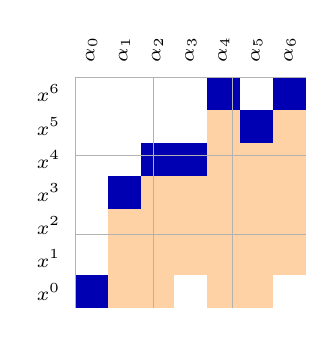
\begin{tikzpicture}[x=4.2mm, y=4.2mm, font=\scriptsize]
  \fill[fill=white] (0,0) rectangle (1,-1);
  \fill[fill=white] (1,0) rectangle (2,-1);
  \fill[fill=white] (2,0) rectangle (3,-1);
  \fill[fill=white] (3,0) rectangle (4,-1);
  \fill[fill=blue!70!black] (4,0) rectangle (5,-1);
  \fill[fill=white] (5,0) rectangle (6,-1);
  \fill[fill=blue!70!black] (6,0) rectangle (7,-1);
  \node[anchor=east] at (-0.15,-0.5) {$x^{6}$};
  \fill[fill=white] (0,-1) rectangle (1,-2);
  \fill[fill=white] (1,-1) rectangle (2,-2);
  \fill[fill=white] (2,-1) rectangle (3,-2);
  \fill[fill=white] (3,-1) rectangle (4,-2);
  \fill[fill=orange!35] (4,-1) rectangle (5,-2);
  \fill[fill=blue!70!black] (5,-1) rectangle (6,-2);
  \fill[fill=orange!35] (6,-1) rectangle (7,-2);
  \node[anchor=east] at (-0.15,-1.5) {$x^{5}$};
  \fill[fill=white] (0,-2) rectangle (1,-3);
  \fill[fill=white] (1,-2) rectangle (2,-3);
  \fill[fill=blue!70!black] (2,-2) rectangle (3,-3);
  \fill[fill=blue!70!black] (3,-2) rectangle (4,-3);
  \fill[fill=orange!35] (4,-2) rectangle (5,-3);
  \fill[fill=orange!35] (5,-2) rectangle (6,-3);
  \fill[fill=orange!35] (6,-2) rectangle (7,-3);
  \node[anchor=east] at (-0.15,-2.5) {$x^{4}$};
  \fill[fill=white] (0,-3) rectangle (1,-4);
  \fill[fill=blue!70!black] (1,-3) rectangle (2,-4);
  \fill[fill=orange!35] (2,-3) rectangle (3,-4);
  \fill[fill=orange!35] (3,-3) rectangle (4,-4);
  \fill[fill=orange!35] (4,-3) rectangle (5,-4);
  \fill[fill=orange!35] (5,-3) rectangle (6,-4);
  \fill[fill=orange!35] (6,-3) rectangle (7,-4);
  \node[anchor=east] at (-0.15,-3.5) {$x^{3}$};
  \fill[fill=white] (0,-4) rectangle (1,-5);
  \fill[fill=orange!35] (1,-4) rectangle (2,-5);
  \fill[fill=orange!35] (2,-4) rectangle (3,-5);
  \fill[fill=orange!35] (3,-4) rectangle (4,-5);
  \fill[fill=orange!35] (4,-4) rectangle (5,-5);
  \fill[fill=orange!35] (5,-4) rectangle (6,-5);
  \fill[fill=orange!35] (6,-4) rectangle (7,-5);
  \node[anchor=east] at (-0.15,-4.5) {$x^{2}$};
  \fill[fill=white] (0,-5) rectangle (1,-6);
  \fill[fill=orange!35] (1,-5) rectangle (2,-6);
  \fill[fill=orange!35] (2,-5) rectangle (3,-6);
  \fill[fill=orange!35] (3,-5) rectangle (4,-6);
  \fill[fill=orange!35] (4,-5) rectangle (5,-6);
  \fill[fill=orange!35] (5,-5) rectangle (6,-6);
  \fill[fill=orange!35] (6,-5) rectangle (7,-6);
  \node[anchor=east] at (-0.15,-5.5) {$x^{1}$};
  \fill[fill=blue!70!black] (0,-6) rectangle (1,-7);
  \fill[fill=orange!35] (1,-6) rectangle (2,-7);
  \fill[fill=orange!35] (2,-6) rectangle (3,-7);
  \fill[fill=white] (3,-6) rectangle (4,-7);
  \fill[fill=orange!35] (4,-6) rectangle (5,-7);
  \fill[fill=orange!35] (5,-6) rectangle (6,-7);
  \fill[fill=white] (6,-6) rectangle (7,-7);
  \node[anchor=east] at (-0.15,-6.5) {$x^{0}$};
  \draw[gray!60, very thin] (0,0) grid (7,-7);
  \node[anchor=west, rotate=90] at (0.5,0.15) {$\alpha_{0}$};
  \node[anchor=west, rotate=90] at (1.5,0.15) {$\alpha_{1}$};
  \node[anchor=west, rotate=90] at (2.5,0.15) {$\alpha_{2}$};
  \node[anchor=west, rotate=90] at (3.5,0.15) {$\alpha_{3}$};
  \node[anchor=west, rotate=90] at (4.5,0.15) {$\alpha_{4}$};
  \node[anchor=west, rotate=90] at (5.5,0.15) {$\alpha_{5}$};
  \node[anchor=west, rotate=90] at (6.5,0.15) {$\alpha_{6}$};
\end{tikzpicture}
\end{minipage}\hfill
  \begin{minipage}[b]{0.62\textwidth}\centering% Sparsity pattern of the Jacobian d[x^d]P_15 / d alpha_i (rows: degree, columns: parameter).
% Characteristic-zero pattern: blue = nonzero constant, orange = nonconstant polynomial, white = zero.
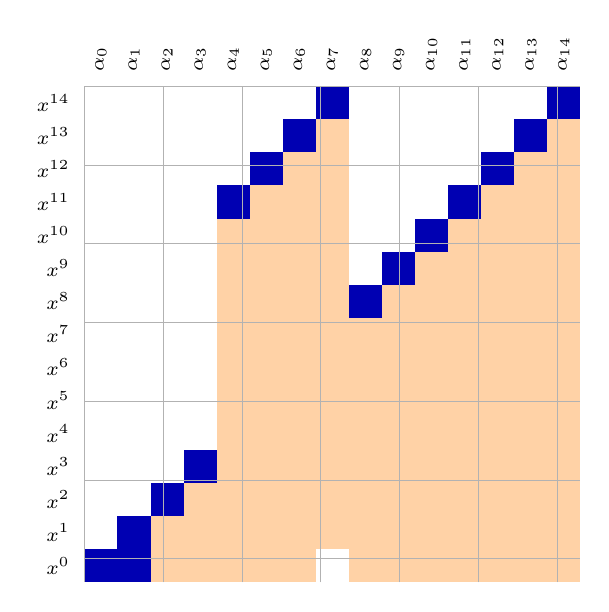
\begin{tikzpicture}[x=4.2mm, y=4.2mm, font=\scriptsize]
  \fill[fill=white] (0,0) rectangle (1,-1);
  \fill[fill=white] (1,0) rectangle (2,-1);
  \fill[fill=white] (2,0) rectangle (3,-1);
  \fill[fill=white] (3,0) rectangle (4,-1);
  \fill[fill=white] (4,0) rectangle (5,-1);
  \fill[fill=white] (5,0) rectangle (6,-1);
  \fill[fill=white] (6,0) rectangle (7,-1);
  \fill[fill=blue!70!black] (7,0) rectangle (8,-1);
  \fill[fill=white] (8,0) rectangle (9,-1);
  \fill[fill=white] (9,0) rectangle (10,-1);
  \fill[fill=white] (10,0) rectangle (11,-1);
  \fill[fill=white] (11,0) rectangle (12,-1);
  \fill[fill=white] (12,0) rectangle (13,-1);
  \fill[fill=white] (13,0) rectangle (14,-1);
  \fill[fill=blue!70!black] (14,0) rectangle (15,-1);
  \node[anchor=east] at (-0.15,-0.5) {$x^{14}$};
  \fill[fill=white] (0,-1) rectangle (1,-2);
  \fill[fill=white] (1,-1) rectangle (2,-2);
  \fill[fill=white] (2,-1) rectangle (3,-2);
  \fill[fill=white] (3,-1) rectangle (4,-2);
  \fill[fill=white] (4,-1) rectangle (5,-2);
  \fill[fill=white] (5,-1) rectangle (6,-2);
  \fill[fill=blue!70!black] (6,-1) rectangle (7,-2);
  \fill[fill=orange!35] (7,-1) rectangle (8,-2);
  \fill[fill=white] (8,-1) rectangle (9,-2);
  \fill[fill=white] (9,-1) rectangle (10,-2);
  \fill[fill=white] (10,-1) rectangle (11,-2);
  \fill[fill=white] (11,-1) rectangle (12,-2);
  \fill[fill=white] (12,-1) rectangle (13,-2);
  \fill[fill=blue!70!black] (13,-1) rectangle (14,-2);
  \fill[fill=orange!35] (14,-1) rectangle (15,-2);
  \node[anchor=east] at (-0.15,-1.5) {$x^{13}$};
  \fill[fill=white] (0,-2) rectangle (1,-3);
  \fill[fill=white] (1,-2) rectangle (2,-3);
  \fill[fill=white] (2,-2) rectangle (3,-3);
  \fill[fill=white] (3,-2) rectangle (4,-3);
  \fill[fill=white] (4,-2) rectangle (5,-3);
  \fill[fill=blue!70!black] (5,-2) rectangle (6,-3);
  \fill[fill=orange!35] (6,-2) rectangle (7,-3);
  \fill[fill=orange!35] (7,-2) rectangle (8,-3);
  \fill[fill=white] (8,-2) rectangle (9,-3);
  \fill[fill=white] (9,-2) rectangle (10,-3);
  \fill[fill=white] (10,-2) rectangle (11,-3);
  \fill[fill=white] (11,-2) rectangle (12,-3);
  \fill[fill=blue!70!black] (12,-2) rectangle (13,-3);
  \fill[fill=orange!35] (13,-2) rectangle (14,-3);
  \fill[fill=orange!35] (14,-2) rectangle (15,-3);
  \node[anchor=east] at (-0.15,-2.5) {$x^{12}$};
  \fill[fill=white] (0,-3) rectangle (1,-4);
  \fill[fill=white] (1,-3) rectangle (2,-4);
  \fill[fill=white] (2,-3) rectangle (3,-4);
  \fill[fill=white] (3,-3) rectangle (4,-4);
  \fill[fill=blue!70!black] (4,-3) rectangle (5,-4);
  \fill[fill=orange!35] (5,-3) rectangle (6,-4);
  \fill[fill=orange!35] (6,-3) rectangle (7,-4);
  \fill[fill=orange!35] (7,-3) rectangle (8,-4);
  \fill[fill=white] (8,-3) rectangle (9,-4);
  \fill[fill=white] (9,-3) rectangle (10,-4);
  \fill[fill=white] (10,-3) rectangle (11,-4);
  \fill[fill=blue!70!black] (11,-3) rectangle (12,-4);
  \fill[fill=orange!35] (12,-3) rectangle (13,-4);
  \fill[fill=orange!35] (13,-3) rectangle (14,-4);
  \fill[fill=orange!35] (14,-3) rectangle (15,-4);
  \node[anchor=east] at (-0.15,-3.5) {$x^{11}$};
  \fill[fill=white] (0,-4) rectangle (1,-5);
  \fill[fill=white] (1,-4) rectangle (2,-5);
  \fill[fill=white] (2,-4) rectangle (3,-5);
  \fill[fill=white] (3,-4) rectangle (4,-5);
  \fill[fill=orange!35] (4,-4) rectangle (5,-5);
  \fill[fill=orange!35] (5,-4) rectangle (6,-5);
  \fill[fill=orange!35] (6,-4) rectangle (7,-5);
  \fill[fill=orange!35] (7,-4) rectangle (8,-5);
  \fill[fill=white] (8,-4) rectangle (9,-5);
  \fill[fill=white] (9,-4) rectangle (10,-5);
  \fill[fill=blue!70!black] (10,-4) rectangle (11,-5);
  \fill[fill=orange!35] (11,-4) rectangle (12,-5);
  \fill[fill=orange!35] (12,-4) rectangle (13,-5);
  \fill[fill=orange!35] (13,-4) rectangle (14,-5);
  \fill[fill=orange!35] (14,-4) rectangle (15,-5);
  \node[anchor=east] at (-0.15,-4.5) {$x^{10}$};
  \fill[fill=white] (0,-5) rectangle (1,-6);
  \fill[fill=white] (1,-5) rectangle (2,-6);
  \fill[fill=white] (2,-5) rectangle (3,-6);
  \fill[fill=white] (3,-5) rectangle (4,-6);
  \fill[fill=orange!35] (4,-5) rectangle (5,-6);
  \fill[fill=orange!35] (5,-5) rectangle (6,-6);
  \fill[fill=orange!35] (6,-5) rectangle (7,-6);
  \fill[fill=orange!35] (7,-5) rectangle (8,-6);
  \fill[fill=white] (8,-5) rectangle (9,-6);
  \fill[fill=blue!70!black] (9,-5) rectangle (10,-6);
  \fill[fill=orange!35] (10,-5) rectangle (11,-6);
  \fill[fill=orange!35] (11,-5) rectangle (12,-6);
  \fill[fill=orange!35] (12,-5) rectangle (13,-6);
  \fill[fill=orange!35] (13,-5) rectangle (14,-6);
  \fill[fill=orange!35] (14,-5) rectangle (15,-6);
  \node[anchor=east] at (-0.15,-5.5) {$x^{9}$};
  \fill[fill=white] (0,-6) rectangle (1,-7);
  \fill[fill=white] (1,-6) rectangle (2,-7);
  \fill[fill=white] (2,-6) rectangle (3,-7);
  \fill[fill=white] (3,-6) rectangle (4,-7);
  \fill[fill=orange!35] (4,-6) rectangle (5,-7);
  \fill[fill=orange!35] (5,-6) rectangle (6,-7);
  \fill[fill=orange!35] (6,-6) rectangle (7,-7);
  \fill[fill=orange!35] (7,-6) rectangle (8,-7);
  \fill[fill=blue!70!black] (8,-6) rectangle (9,-7);
  \fill[fill=orange!35] (9,-6) rectangle (10,-7);
  \fill[fill=orange!35] (10,-6) rectangle (11,-7);
  \fill[fill=orange!35] (11,-6) rectangle (12,-7);
  \fill[fill=orange!35] (12,-6) rectangle (13,-7);
  \fill[fill=orange!35] (13,-6) rectangle (14,-7);
  \fill[fill=orange!35] (14,-6) rectangle (15,-7);
  \node[anchor=east] at (-0.15,-6.5) {$x^{8}$};
  \fill[fill=white] (0,-7) rectangle (1,-8);
  \fill[fill=white] (1,-7) rectangle (2,-8);
  \fill[fill=white] (2,-7) rectangle (3,-8);
  \fill[fill=white] (3,-7) rectangle (4,-8);
  \fill[fill=orange!35] (4,-7) rectangle (5,-8);
  \fill[fill=orange!35] (5,-7) rectangle (6,-8);
  \fill[fill=orange!35] (6,-7) rectangle (7,-8);
  \fill[fill=orange!35] (7,-7) rectangle (8,-8);
  \fill[fill=orange!35] (8,-7) rectangle (9,-8);
  \fill[fill=orange!35] (9,-7) rectangle (10,-8);
  \fill[fill=orange!35] (10,-7) rectangle (11,-8);
  \fill[fill=orange!35] (11,-7) rectangle (12,-8);
  \fill[fill=orange!35] (12,-7) rectangle (13,-8);
  \fill[fill=orange!35] (13,-7) rectangle (14,-8);
  \fill[fill=orange!35] (14,-7) rectangle (15,-8);
  \node[anchor=east] at (-0.15,-7.5) {$x^{7}$};
  \fill[fill=white] (0,-8) rectangle (1,-9);
  \fill[fill=white] (1,-8) rectangle (2,-9);
  \fill[fill=white] (2,-8) rectangle (3,-9);
  \fill[fill=white] (3,-8) rectangle (4,-9);
  \fill[fill=orange!35] (4,-8) rectangle (5,-9);
  \fill[fill=orange!35] (5,-8) rectangle (6,-9);
  \fill[fill=orange!35] (6,-8) rectangle (7,-9);
  \fill[fill=orange!35] (7,-8) rectangle (8,-9);
  \fill[fill=orange!35] (8,-8) rectangle (9,-9);
  \fill[fill=orange!35] (9,-8) rectangle (10,-9);
  \fill[fill=orange!35] (10,-8) rectangle (11,-9);
  \fill[fill=orange!35] (11,-8) rectangle (12,-9);
  \fill[fill=orange!35] (12,-8) rectangle (13,-9);
  \fill[fill=orange!35] (13,-8) rectangle (14,-9);
  \fill[fill=orange!35] (14,-8) rectangle (15,-9);
  \node[anchor=east] at (-0.15,-8.5) {$x^{6}$};
  \fill[fill=white] (0,-9) rectangle (1,-10);
  \fill[fill=white] (1,-9) rectangle (2,-10);
  \fill[fill=white] (2,-9) rectangle (3,-10);
  \fill[fill=white] (3,-9) rectangle (4,-10);
  \fill[fill=orange!35] (4,-9) rectangle (5,-10);
  \fill[fill=orange!35] (5,-9) rectangle (6,-10);
  \fill[fill=orange!35] (6,-9) rectangle (7,-10);
  \fill[fill=orange!35] (7,-9) rectangle (8,-10);
  \fill[fill=orange!35] (8,-9) rectangle (9,-10);
  \fill[fill=orange!35] (9,-9) rectangle (10,-10);
  \fill[fill=orange!35] (10,-9) rectangle (11,-10);
  \fill[fill=orange!35] (11,-9) rectangle (12,-10);
  \fill[fill=orange!35] (12,-9) rectangle (13,-10);
  \fill[fill=orange!35] (13,-9) rectangle (14,-10);
  \fill[fill=orange!35] (14,-9) rectangle (15,-10);
  \node[anchor=east] at (-0.15,-9.5) {$x^{5}$};
  \fill[fill=white] (0,-10) rectangle (1,-11);
  \fill[fill=white] (1,-10) rectangle (2,-11);
  \fill[fill=white] (2,-10) rectangle (3,-11);
  \fill[fill=white] (3,-10) rectangle (4,-11);
  \fill[fill=orange!35] (4,-10) rectangle (5,-11);
  \fill[fill=orange!35] (5,-10) rectangle (6,-11);
  \fill[fill=orange!35] (6,-10) rectangle (7,-11);
  \fill[fill=orange!35] (7,-10) rectangle (8,-11);
  \fill[fill=orange!35] (8,-10) rectangle (9,-11);
  \fill[fill=orange!35] (9,-10) rectangle (10,-11);
  \fill[fill=orange!35] (10,-10) rectangle (11,-11);
  \fill[fill=orange!35] (11,-10) rectangle (12,-11);
  \fill[fill=orange!35] (12,-10) rectangle (13,-11);
  \fill[fill=orange!35] (13,-10) rectangle (14,-11);
  \fill[fill=orange!35] (14,-10) rectangle (15,-11);
  \node[anchor=east] at (-0.15,-10.5) {$x^{4}$};
  \fill[fill=white] (0,-11) rectangle (1,-12);
  \fill[fill=white] (1,-11) rectangle (2,-12);
  \fill[fill=white] (2,-11) rectangle (3,-12);
  \fill[fill=blue!70!black] (3,-11) rectangle (4,-12);
  \fill[fill=orange!35] (4,-11) rectangle (5,-12);
  \fill[fill=orange!35] (5,-11) rectangle (6,-12);
  \fill[fill=orange!35] (6,-11) rectangle (7,-12);
  \fill[fill=orange!35] (7,-11) rectangle (8,-12);
  \fill[fill=orange!35] (8,-11) rectangle (9,-12);
  \fill[fill=orange!35] (9,-11) rectangle (10,-12);
  \fill[fill=orange!35] (10,-11) rectangle (11,-12);
  \fill[fill=orange!35] (11,-11) rectangle (12,-12);
  \fill[fill=orange!35] (12,-11) rectangle (13,-12);
  \fill[fill=orange!35] (13,-11) rectangle (14,-12);
  \fill[fill=orange!35] (14,-11) rectangle (15,-12);
  \node[anchor=east] at (-0.15,-11.5) {$x^{3}$};
  \fill[fill=white] (0,-12) rectangle (1,-13);
  \fill[fill=white] (1,-12) rectangle (2,-13);
  \fill[fill=blue!70!black] (2,-12) rectangle (3,-13);
  \fill[fill=orange!35] (3,-12) rectangle (4,-13);
  \fill[fill=orange!35] (4,-12) rectangle (5,-13);
  \fill[fill=orange!35] (5,-12) rectangle (6,-13);
  \fill[fill=orange!35] (6,-12) rectangle (7,-13);
  \fill[fill=orange!35] (7,-12) rectangle (8,-13);
  \fill[fill=orange!35] (8,-12) rectangle (9,-13);
  \fill[fill=orange!35] (9,-12) rectangle (10,-13);
  \fill[fill=orange!35] (10,-12) rectangle (11,-13);
  \fill[fill=orange!35] (11,-12) rectangle (12,-13);
  \fill[fill=orange!35] (12,-12) rectangle (13,-13);
  \fill[fill=orange!35] (13,-12) rectangle (14,-13);
  \fill[fill=orange!35] (14,-12) rectangle (15,-13);
  \node[anchor=east] at (-0.15,-12.5) {$x^{2}$};
  \fill[fill=white] (0,-13) rectangle (1,-14);
  \fill[fill=blue!70!black] (1,-13) rectangle (2,-14);
  \fill[fill=orange!35] (2,-13) rectangle (3,-14);
  \fill[fill=orange!35] (3,-13) rectangle (4,-14);
  \fill[fill=orange!35] (4,-13) rectangle (5,-14);
  \fill[fill=orange!35] (5,-13) rectangle (6,-14);
  \fill[fill=orange!35] (6,-13) rectangle (7,-14);
  \fill[fill=orange!35] (7,-13) rectangle (8,-14);
  \fill[fill=orange!35] (8,-13) rectangle (9,-14);
  \fill[fill=orange!35] (9,-13) rectangle (10,-14);
  \fill[fill=orange!35] (10,-13) rectangle (11,-14);
  \fill[fill=orange!35] (11,-13) rectangle (12,-14);
  \fill[fill=orange!35] (12,-13) rectangle (13,-14);
  \fill[fill=orange!35] (13,-13) rectangle (14,-14);
  \fill[fill=orange!35] (14,-13) rectangle (15,-14);
  \node[anchor=east] at (-0.15,-13.5) {$x^{1}$};
  \fill[fill=blue!70!black] (0,-14) rectangle (1,-15);
  \fill[fill=blue!70!black] (1,-14) rectangle (2,-15);
  \fill[fill=orange!35] (2,-14) rectangle (3,-15);
  \fill[fill=orange!35] (3,-14) rectangle (4,-15);
  \fill[fill=orange!35] (4,-14) rectangle (5,-15);
  \fill[fill=orange!35] (5,-14) rectangle (6,-15);
  \fill[fill=orange!35] (6,-14) rectangle (7,-15);
  \fill[fill=white] (7,-14) rectangle (8,-15);
  \fill[fill=orange!35] (8,-14) rectangle (9,-15);
  \fill[fill=orange!35] (9,-14) rectangle (10,-15);
  \fill[fill=orange!35] (10,-14) rectangle (11,-15);
  \fill[fill=orange!35] (11,-14) rectangle (12,-15);
  \fill[fill=orange!35] (12,-14) rectangle (13,-15);
  \fill[fill=orange!35] (13,-14) rectangle (14,-15);
  \fill[fill=orange!35] (14,-14) rectangle (15,-15);
  \node[anchor=east] at (-0.15,-14.5) {$x^{0}$};
  \draw[gray!60, very thin] (0,0) grid (15,-15);
  \node[anchor=west, rotate=90] at (0.5,0.15) {$\alpha_{0}$};
  \node[anchor=west, rotate=90] at (1.5,0.15) {$\alpha_{1}$};
  \node[anchor=west, rotate=90] at (2.5,0.15) {$\alpha_{2}$};
  \node[anchor=west, rotate=90] at (3.5,0.15) {$\alpha_{3}$};
  \node[anchor=west, rotate=90] at (4.5,0.15) {$\alpha_{4}$};
  \node[anchor=west, rotate=90] at (5.5,0.15) {$\alpha_{5}$};
  \node[anchor=west, rotate=90] at (6.5,0.15) {$\alpha_{6}$};
  \node[anchor=west, rotate=90] at (7.5,0.15) {$\alpha_{7}$};
  \node[anchor=west, rotate=90] at (8.5,0.15) {$\alpha_{8}$};
  \node[anchor=west, rotate=90] at (9.5,0.15) {$\alpha_{9}$};
  \node[anchor=west, rotate=90] at (10.5,0.15) {$\alpha_{10}$};
  \node[anchor=west, rotate=90] at (11.5,0.15) {$\alpha_{11}$};
  \node[anchor=west, rotate=90] at (12.5,0.15) {$\alpha_{12}$};
  \node[anchor=west, rotate=90] at (13.5,0.15) {$\alpha_{13}$};
  \node[anchor=west, rotate=90] at (14.5,0.15) {$\alpha_{14}$};
\end{tikzpicture}
\end{minipage}
  \caption{Sparsity pattern of the Jacobian $\partial\,\coeff{P_n}{d}/\partial\alpha_i$ for the septic base $P_7$ (left) and the special case $P_{15}$ (right); rows are degrees $d=n-1,\ldots,0$ and columns are parameters.
  Blue (dark) cells are nonzero field constants, orange (light) cells are non-constant polynomials in the parameters, white cells are zero.
  Decoding proceeds top-down: each row exposes one fresh parameter with a constant slope once the parameters of the rows above are known.
  Where a row contains two constant cells (e.g.\ $\coeff{P_7}{6}$, which involves $\alpha_4$ and $\alpha_6$), the decoder first recovers an internal quantity of the construction (here $z_2=\alpha_4+1+\alpha_6$) and separates the two parameters at a lower row; this is the composition structure that the compatible-pair lemmas make precise.}
  \label{fig:jacobian-pattern}
\end{figure}

\Cref{fig:jacobian-pattern} is only a visualization of the explicit pivot order.  We do
not infer invertibility from a Jacobian determinant; every inverse used below
is supplied by the coefficient recurrences themselves.

\paragraph{Constructive viewpoint.}
Compatibility is a \emph{causal} recovery condition.  At cutoff $j$, the
decoder for $[x^j]P^{(1)}$ may use only coefficients of
$\Phi=xP^{(1)}+P^{(2)}$ in degrees at least $j+1$, and the decoder for
$[x^j]P^{(2)}$ may use only degrees at least $j$.  In particular, mere
recoverability of the pair from the whole window is not sufficient.  The
closure proofs below preserve this cutoff condition because all their
reconstructions run in descending degree order.

Thus a proof of compatibility must provide a cutoff-respecting decoder, not
merely recover both components from the entire window.  We will usually give
that decoder as a descending pivot table.  The following stronger form is
tailored to the $T_{k,2^l}$ remainder recursion.

\begin{definition}[Coefficient-triangular remainder pair]
\label{def:coefficient-triangular}
Let $d\ge0$, let $\alpha_0,\ldots,\alpha_{d-1}$ be the active parameters, and
let $K$ be the quantities already known to the decoder.  A pair
$(R^{(1)},R^{(2)})$ is \emph{coefficient-triangular} if, for every
$j\in\rng d$,
\begin{align}
 [x^j]R^{(1)}
   &\polyfrom (K;\alpha_{j+1},\ldots,\alpha_{d-1}),&
 [x^j]R^{(2)}
   &\polyfrom (K;\alpha_j,\ldots,\alpha_{d-1}),
   \label{eq:filtered-remainder}\\
 [x^j](xR^{(1)}+R^{(2)})
   &=\lambda_j\alpha_j+F_j,
   &F_j&\polyfrom (K;\alpha_{j+1},\ldots,\alpha_{d-1}).
   \label{eq:filtered-pivot}
\end{align}
Every pivot slope $\lambda_j$ is required to lie in $\mathbb F^\times$.
Coefficients in degrees at least $d$ are required to be polynomially
recoverable from $K$ alone.
\end{definition}

\begin{lemma}[A triangular remainder pair is causal]
\label{lem:triangular-implies-compatible}
Let $H,\widetilde H$ be auxiliary monic polynomials of degree $h$, let
$N=kh$ and $d=(k-1)h$, and set
\[
 T^{(1)}=H^k+R^{(1)},\qquad
 T^{(2)}=\widetilde H^k+R^{(2)}.
\]
If $(R^{(1)},R^{(2)})$ is coefficient-triangular and has degree at most $d$,
then the parameters are recovered from
$D=xR^{(1)}+R^{(2)}$ by descending induction, and
$(T^{(1)},T^{(2)})$ is compatible on $\rng d$ given
$(H,\widetilde H)$ and the other auxiliary data.
\end{lemma}
\begin{proof}
Equation~\eqref{eq:filtered-pivot} is a descending decoder: after
$\alpha_{j+1},\ldots,\alpha_{d-1}$ have been recovered, divide by the fixed
nonzero scalar $\lambda_j$ to recover $\alpha_j$.  The support conditions in
\eqref{eq:filtered-remainder} say that $[x^j]R^{(1)}$ uses only the already
recovered parameters with index at least $j+1$, while $[x^j]R^{(2)}$ may also
use $\alpha_j$.  Coefficients in degrees at least $d$ are known from $K$.
Finally
\[
 D=xT^{(1)}+T^{(2)}-\bigl(xH^k+\widetilde H^k\bigr),
\]
so the same cutoff statements hold with the coefficients of
$xT^{(1)}+T^{(2)}$.  This is precisely compatibility.
\end{proof}

\begin{lemma}[Shifting a triangular remainder block]
\label{lem:triangular-shift}
Let $(A^{(1)},A^{(2)})$ be coefficient-triangular for active
parameters $\eta_0,\ldots,\eta_{e-1}$, given known data $K$.
Let $L_1,L_2$ be monic polynomials of the same degree $h$.  Replace $\eta_i$
by a parameter $\alpha_{h+i}$.  The coefficients of $L_1,L_2$ may either be
included in the known data $K$, or be polynomially recoverable from
\[
       (K;\zeta_1,\ldots,\zeta_s),
\]
where every $\zeta_u$ has been assigned a global parameter index at least
$h+e$.  Thus the $\zeta$'s belong to a block higher than the block being
shifted.  Then the pair

\[
       (L_1A^{(1)},L_2A^{(2)})
\]

has the triangular support conditions on the shifted block
$h,\ldots,h+e-1$, and its combined pivot at $h+i$ is the old pivot at
$i$.  More precisely, coefficients below $h+e$ have no active parameter
of index smaller than their degree (with the usual one-degree offset for
the first component), and

\[
 [x^{h+i}](xL_1A^{(1)}+L_2A^{(2)})
   =\lambda_i\alpha_{h+i}+F_{h+i},
   \qquad F_{h+i}\polyfrom
      (K;\zeta_1,\ldots,\zeta_s,\alpha_{h+i+1},\ldots).
\]

The assertion remains true after adding polynomials whose coefficients are
polynomially recoverable from $(K;\zeta_1,\ldots,\zeta_s)$, provided their
active parameters also have global indices at least $h+e$.
\end{lemma}
\begin{proof}
Write $A^{(1)}_q=[x^q]A^{(1)}$ and similarly for $A^{(2)}$.  By
coefficient-triangularity, $A^{(1)}_q$ is polynomially recoverable from
$(K;\eta_{q+1},\ldots,\eta_{e-1})$, while $A^{(2)}_q$ is polynomially
recoverable from $(K;\eta_q,\ldots,\eta_{e-1})$.
In a coefficient of $L_rA^{(r)}$, a summand has the form
$L_{r,t}A^{(r)}_q$ with $t+q=j$ and $0\le t\le h$.  Thus a parameter
$\eta_i$ occurring in the first (respectively second) component can occur
only when $j\le h+i-1$ (respectively $j\le h+i$), which is exactly the
required support after reindexing.
For the coefficient of degree $h+i$ in the combined polynomial, the
summands with $t=h$ are
$A^{(1)}_{i-1}+A^{(2)}_i$, because both factors are monic.  All summands
with $t<h$ involve only $A^{(1)}_q$ with $q>i-1$ or $A^{(2)}_q$ with
$q>i$, hence only parameters of index strictly larger than $i$.  The old
    pivot formula therefore gives the displayed new pivot with the same
    $\lambda_i$.  Substituting the formulas for the coefficients of
    $L_1,L_2$ introduces only the higher parameters $\zeta_u$, whose global
    indices are at least $h+e$ and hence are strictly larger than every
    index in the shifted block.  The same observation applies to the allowed
    auxiliary additions, so neither the support nor the pivot is changed.

The support assertion is only needed on the shifted block
$h,\ldots,h+e-1$.  Rows below $h$ can of course contain the low
coefficients of the inner pair (the multiplier $L_r$ need not be a
monomial); this is not a violation, since every active parameter there has
index at least $h$.  Once the shifted block has been decoded, those low
rows are known polynomials and can be subtracted when the remaining
low-degree rows are processed.
\end{proof}

\begin{lemma}[Concatenating triangular blocks]
\label{lem:triangular-block-concatenation}
Let the active parameters be partitioned into consecutive blocks
\[
  I_r=\{b_r,\ldots,b_{r+1}-1\},\qquad
  0=b_0<b_1<\cdots<b_s=d.
\]
Suppose that, for every $r$, the coefficient and pivot formulas on the rows
$j\in I_r$ have been proved with a finite side list $Y_r$, in the form
\[
\begin{aligned}
 [x^j]R^{(1)}&\polyfrom
   (Y_r;\alpha_{j+1},\ldots,\alpha_{b_{r+1}-1}),\\
 [x^j]R^{(2)}&\polyfrom
   (Y_r;\alpha_j,\ldots,\alpha_{b_{r+1}-1}),\\
 [x^j](xR^{(1)}+R^{(2)})
   &=\lambda_j\alpha_j+F_j,
 \qquad F_j\polyfrom
   (Y_r;\alpha_{j+1},\ldots,\alpha_{b_{r+1}-1}),
\end{aligned}
\]
where each $\lambda_j\in\mathbb F^\times$, and suppose moreover that every
entry of $Y_r$ is polynomially recoverable from
\[
       (K;\alpha_{b_{r+1}},\ldots,\alpha_{d-1}).
\]
Then the whole pair is coefficient-triangular for
$(\alpha_0,\ldots,\alpha_{d-1})$ given $K$.

In particular, a quantity which has been decoded in a higher block may be
treated as known while proving a lower block: substituting its polynomial
formula only introduces parameters with strictly larger global indices.
\end{lemma}
\begin{proof}
Substitute the displayed formulas for the entries of $Y_r$.  For a row
$j\in I_r$, all parameters occurring in the substituted side list have
index at least $b_{r+1}>j$, while the explicitly displayed parameters have
index at least $j$ (and at least $j+1$ in the first component and in the
remainder term $F_j$).  The three resulting formulas are therefore exactly
the three formulas in \Cref{def:coefficient-triangular}.  Processing the
blocks in the order $I_{s-1},\ldots,I_0$ gives the descending decoder.
\end{proof}

\paragraph{How the tables compose.}
The closure lemmas below prove their own cutoffs by descending induction.
Within the $T$ recursion, \Cref{lem:triangular-shift} transports a block
through overlapping monic factors, and
\Cref{lem:triangular-block-concatenation} joins consecutive blocks.  After an
intermediate polynomial has been recovered, all later uses of it are ordinary
substitution as in \Cref{lem:extractable-via-derivable}; no separate causal
composition principle is used.

\paragraph{Stage-table convention.}
Every stage table is read from its highest row downward.  A line with row set
$I$, active block $(\alpha_j)_{j\in I}$, and slope $\lambda$ abbreviates the
three assertions, for each $j\in I$,
\[
\begin{aligned}
 [x^j]R^{(1)}&\polyfrom(K;\alpha_{>j}),&
 [x^j]R^{(2)}&\polyfrom(K;\alpha_{\ge j}),\\
 [x^j](xR^{(1)}+R^{(2)})
   &=\lambda\alpha_j+F_j(K;\alpha_{>j}).
\end{aligned}
\]
The source column identifies the term producing the pivot.  The text beside
the table verifies that all other occurrences lie in lower rows or involve
only higher parameters.  Once the listed row sets partition the parameter
range, \Cref{lem:triangular-block-concatenation} turns the table into the
coefficient-triangular invariant.  Thus the tables are compact decoder
proofs, not coefficient-pattern heuristics; \Cref{fig:triangular-blocks}
draws the two moves.

\begin{figure}[H]
  \centering
  \resizebox{\textwidth}{!}{% The two structural operations used to assemble coefficient-triangular tables.
\begin{tikzpicture}[x=1cm,y=1cm,>=Latex]
  \node[fp panel title] at (0,4.1) {(a) Shift through a monic factor};
  \node[fp active, minimum width=42mm] (old) at (2.15,2.55)
    {old parameters $\eta_{e-1},\ldots,\eta_0$};
  \node[fp known, minimum width=24mm] (factor) at (2.15,3.42)
    {$L=x^h+\cdots$};
  \node[fp label, right=1mm of factor] {leading coefficient $1$};
  \node[fp active, minimum width=42mm] (shifted) at (1.55,1.05)
    {reindexed $\alpha_{h+e-1},\ldots,\alpha_h$};
  \node[fp unread, minimum width=16mm, right=0pt of shifted]
    {rows $<h$};
  \draw[fp decode] (old.south) -- node[fp label, right]
    {$\times L$: shift by $h$} (shifted.north);
  \node[fp label, anchor=west, text=fpBlue!80!black] at (0,0.22)
    {monicity preserves every pivot slope $\lambda_i$};

  \node[fp panel title] at (7.15,4.1) {(b) Concatenate descending blocks};
  \draw[fp decode] (7.15,3.42) -- node[fp label, above]
    {decoding order} (13.55,3.42);
  \node[fp active, minimum width=22mm, anchor=west] (tail) at (7.15,2.55)
    {new tail};
  \node[fp recursive, minimum width=27mm, anchor=west] (inner) at (9.35,2.55)
    {shifted recursion};
  \node[fp second, minimum width=18mm, anchor=west] (low) at (12.05,2.55)
    {low block};
  \draw[fp dependence] (tail.south) to[bend right=12]
    node[fp label, below] {decoded side data} (inner.south);
  \draw[fp dependence] (inner.south) to[bend right=12] (low.south);
  \node[fp label] at (8.25,1.18)
    {$I_{s-1}$ decoded first};
  \node[fp label] at (10.7,1.18)
    {then $I_{s-2},\ldots$};
  \node[fp label] at (12.95,1.18)
    {finally $I_0$};
  \node[fp label, anchor=west, text=fpBlue!80!black] at (7.15,0.22)
    {higher-block formulas may be substituted into every lower block};
\end{tikzpicture}
}
  \caption{The two structural moves behind the stage tables (styles as
  keyed in \Cref{fig:decoder-language}).
  Multiplication by a monic degree-$h$ factor shifts an inner triangular
  block by $h$ rows without changing its pivot slopes; lower rows may contain
  that block but are processed only after it is known.  Consecutive blocks
  are then decoded from high degree to low degree, with each completed block
  becoming legitimate side information for the next.  This is the preceding
  shifting and concatenation calculus in pictures.}
  \label{fig:triangular-blocks}
\end{figure}


\subsection{Causal closure and top-window calculus}

The three closure operations used later have the same shape.  Their window
conditions ensure that each observed row belongs to at most one unresolved
input block; monicity then supplies a constant pivot.
\[
\begin{array}{c|c|c}
  \text{operation}&\text{output window}&\text{descending step}\\ \hline
  \text{sum}&G_1\cup G_2&\text{subtract the other input row}\\
  \text{product}&(n_2+G_1)\cup(n_1+G_2)
    &\text{peel the monic Cauchy boundary}\\
  \text{square}&n+G&\Psi_{n+i}=2\Phi_i+\text{higher terms}
\end{array}
\]
The proofs below establish the exact first- and second-component cutoffs; the
table is only a map of those proofs, and \Cref{fig:causal-closures} pictures
the closure moves.

\begin{figure}[H]
  \centering
  \resizebox{\textwidth}{!}{% Window geometry for the three closure operations on compatible pairs.
\begin{tikzpicture}[x=1cm,y=1cm,>=Latex]
  \node[fp panel title] at (0,3.2) {(a) Sum};
  \node[fp active, minimum width=15mm, anchor=west] at (0,2.43) {$G_1$};
  \node[fp unread, minimum width=8mm, anchor=west] at (1.5,2.43) {};
  \node[fp active, minimum width=10mm, anchor=west] at (2.3,2.43) {$G_1$};
  \node[fp second, minimum width=8mm, anchor=west] at (1.5,1.73) {$G_2$};
  \node[fp second, minimum width=13mm, anchor=west] at (3.3,1.73) {$G_2$};
  \node[fp label, anchor=west] at (0,1.05) {$G_1\cap G_2=\emptyset$};
  \draw[fp decode] (0,0.64) -- node[fp label, above]
    {high degree to low degree} (4.6,0.64);
  \node[fp label, anchor=west] at (0,0.2) {one unresolved input per row};

  \node[fp panel title] at (4.85,3.2) {(b) Product};
  \node[fp active, minimum width=19mm, anchor=west] (g1) at (5.25,2.43) {$G_1$};
  \node[fp second, minimum width=19mm, anchor=west] (g2) at (7.35,2.43) {$G_2$};
  \node[fp active, minimum width=19mm, anchor=west] (sg1) at (4.85,1.35) {$n_2+G_1$};
  \node[fp second, minimum width=19mm, anchor=west] (sg2) at (7.0,1.35) {$n_1+G_2$};
  \draw[fp flow] (g1.south) -- node[fp label, right=1.5mm] {$+n_2$} (sg1.north);
  \draw[fp flow] (g2.south) -- node[fp label, right=1.5mm] {$+n_1$} (sg2.north);
  \node[fp label, anchor=west] at (4.85,0.72) {shifted windows disjoint};
  \node[fp label, anchor=west] at (4.85,0.2) {peel the monic Cauchy boundary};

  \node[fp panel title] at (9.9,3.2) {(c) Square};
  \node[fp active, minimum width=25mm, anchor=west] (gin) at (11.25,2.43) {input $G$};
  \node[fp active, minimum width=25mm, anchor=west] (gout) at (9.9,1.35) {output $n+G$};
  \draw[fp decode] (gin.south) -- (gout.north);
  \node[fp label, anchor=east] at (11.1,1.95) {shift by $n$};
  \node[fp label, anchor=west] at (9.9,0.72)
    {$\coeff{\Psi}{n+i}=2\coeff{\Phi}{i}+F_i$};
  \node[fp label, anchor=west] at (9.9,0.2)
    {pivot $2$ ($\operatorname{char}\mathbb F\ne2$)};
\end{tikzpicture}
}
  \caption{Window geometry of the three causal closure operations.  A sum
  uses disjoint observed rows; a product translates each input window by the
  degree of the other monic factor; and a square translates the window by
  the common degree and exposes the old row with slope~$2$.  In every case
  the output descent encounters at most one unresolved input row.}
  \label{fig:causal-closures}
\end{figure}

\begin{lemma}[Additivity of Compatible Pairs]
    Let $(P^{(1)}_1, P^{(2)}_1), (P^{(1)}_2, P^{(2)}_2) \in \mathbb{F}[x]^2$ be compatible pairs on $G_1 \subseteq \idx{n_1}$ and $G_2 \subseteq \idx{n_2}$ given $(B_k)_{k \in [t]}$, respectively, with $\deg P^{(1)}_1 = n_1$ and $\deg P^{(1)}_2 = n_2$.
    Assume $G_1 \cap G_2 = \emptyset$. If $n_1 \ne n_2$, define
    \[
        (P^{(1)},P^{(2)}) \coloneqq (P^{(1)}_1 + P^{(1)}_2,\; P^{(2)}_1 + P^{(2)}_2).
    \]
    If instead $n_1 = n_2$, define
    \[
        (P^{(1)},P^{(2)}) \coloneqq \bigl(P^{(1)}_1 + P^{(1)}_2 - x^{n_1},\; P^{(2)}_1 + P^{(2)}_2 - x^{n_1}\bigr).
    \]
    Then $(P^{(1)}, P^{(2)})$ is a compatible pair on $G_1 \cup G_2$ given $(B_k)_{k \in [t]}$, and $P^{(1)}_1, P^{(2)}_1, P^{(1)}_2, P^{(2)}_2$ are all derivable from $(P^{(1)}, P^{(2)}, (B_k)_{k \in [t]})$.
\end{lemma}
\begin{proof}
    For $i\in\{1,2\}$ define $\Phi_i(x)\coloneqq xP^{(1)}_i(x)+P^{(2)}_i(x)$, and adopt the convention $\coeff{P^{(1)}_i}{-1}=0$.
    Define
    \[
        \Delta(x)\coloneqq
        \begin{cases}
            0 & \text{if } n_1\ne n_2,\\
            x^{n_1+1}+x^{n_1} & \text{if } n_1=n_2.
        \end{cases}
    \]
    Then the combined polynomial for $(P^{(1)},P^{(2)})$ satisfies
    \[
        xP^{(1)}(x)+P^{(2)}(x)=\Phi_1(x)+\Phi_2(x)-\Delta(x).
    \]

    Set $G\coloneqq G_1\cup G_2$. From $\bigl(\coeff{xP^{(1)}+P^{(2)}}{d}\bigr)_{d\in G}$ we can recover $\bigl(\coeff{\Phi_1+\Phi_2}{d}\bigr)_{d\in G}$ by adding the known coefficients of $\Delta$.
    We now show that from the coefficients $\bigl(\coeff{\Phi_1+\Phi_2}{d}\bigr)_{d\in G}$ (and the coefficients of $(B_k)_{k\in[t]}$) we can recover $\bigl(\coeff{\Phi_1}{d}\bigr)_{d\in G_1}$ and $\bigl(\coeff{\Phi_2}{d}\bigr)_{d\in G_2}$.
    We proceed by descending induction on $d$, starting above
    $\max(n_1,n_2)+1$.  Initialize
    \[
      \coeff{\Phi_i}{d}=0\quad(d>n_i+1),\qquad
      \coeff{\Phi_i}{n_i+1}=1.
    \]
    At a row $d\le n_i$ outside $G_i$, compatibility of the $i$th input pair
    expresses $\coeff{P^{(1)}_i}{d-1}$ in terms of its higher
    $\Phi_i$-rows (with $\coeff{P^{(1)}_i}{-1}=0$).  It does the same for
    $\coeff{P^{(2)}_i}{d}$ when $d<n_i$, while for $d=n_i$ that coefficient
    is the known leading~$1$.  Hence it determines
    \[
      \coeff{\Phi_i}{d}
       =\coeff{P^{(1)}_i}{d-1}+\coeff{P^{(2)}_i}{d}.
    \]
    The leading coefficient at $d=n_i+1$ and the zero rows above it are
    supplied by monicity, so no unobserved row is used.

    If $d\in G_1$ (so $d\notin G_2$), then $d\in G$ and we can compute
    \[
        \coeff{\Phi_1}{d}=\coeff{\Phi_1+\Phi_2}{d}-\coeff{\Phi_2}{d}.
    \]
    The case $d\in G_2$ is symmetric.
    Finally, if $d\notin G_1\cup G_2$ then both $d\notin G_1$ and $d\notin G_2$, so compatibility of each pair determines $\coeff{\Phi_1}{d}$ and $\coeff{\Phi_2}{d}$ from higher coefficients and $(B_k)_{k\in[t]}$ without using $\coeff{\Phi_1+\Phi_2}{d}$.

    This completes the induction and thus recovers the required coefficients of $\Phi_1$ on $G_1$ and $\Phi_2$ on $G_2$.
    Applying compatibility of each original pair, we can recover all coefficients of $P^{(1)}_1,P^{(2)}_1$ from $(\coeff{\Phi_1}{d})_{d\in G_1}$ and $(B_k)_{k\in[t]}$, and similarly for $P^{(1)}_2,P^{(2)}_2$.
    Therefore $P^{(1)}_1,P^{(2)}_1,P^{(1)}_2,P^{(2)}_2$ are derivable from $(P^{(1)},P^{(2)},(B_k)_{k\in[t]})$.
    We record the information cutoff explicitly.  The induction just given has
    the following invariant: for every $r$, each input coefficient
    $\coeff{\Phi_i}{r}$ that is used is a polynomial in the auxiliary data and
    in output coefficients $\coeff{\Phi}{s}$ with $s\in G$ and $s\ge r$.
    Indeed, at a row $r\in G_i$ we read the output row $r$, while at a row
    outside $G_i$ the compatibility formula for the $i$th input uses only
    rows strictly above $r$; the latter are handled recursively.  The known
    correction $\Delta$ does not change this invariant.

    To recover $\coeff{P^{(1)}}{j}$, apply the two input compatibility formulas
    only at rows $r\ge j+1$.  The invariant then uses output rows $s\ge r\ge
    j+1$.  For $\coeff{P^{(2)}}{j}$ the corresponding rows satisfy $r\ge j$,
    and hence use only output rows $s\ge j$.  Thus the output pair is
    compatible on $G$ with exactly the two cutoffs in
    \Cref{def:compatible-pair}, not merely recoverable from the whole window.
\end{proof}

\begin{lemma}[Multiplicativity of Compatible Pairs]
    Let $(P^{(1)}_1, P^{(2)}_1), (P^{(1)}_2, P^{(2)}_2) \in \mathbb{F}[x]^2$ be compatible pairs on $G_1 \subseteq \idx{n_1}$ and $G_2 \subseteq \idx{n_2}$ given $(B_k)_{k \in [t]}$, respectively, with $\deg P^{(1)}_1 = n_1$ and $\deg P^{(1)}_2 = n_2$.
    If $(n_2 + G_1) \cap (n_1 + G_2) = \emptyset$ then $(P^{(1)}_1 \cdot P^{(1)}_2, P^{(2)}_1 \cdot P^{(2)}_2)$ is a compatible pair on $(n_2 + G_1) \cup (n_1 + G_2)$ given $(B_k)_{k \in [t]}$, and $P^{(1)}_1, P^{(2)}_1, P^{(1)}_2, P^{(2)}_2$ are all derivable from $(P^{(1)}_1 \cdot P^{(1)}_2, P^{(2)}_1 \cdot P^{(2)}_2, (B_k)_{k \in [t]})$.
\end{lemma}
\begin{proof}
    Define $\Phi_i(x)\coloneqq xP^{(1)}_i(x)+P^{(2)}_i(x)$ for $i\in\{1,2\}$ and
    \[
        \Phi(x)\coloneqq x\bigl(P^{(1)}_1(x)P^{(1)}_2(x)\bigr)+P^{(2)}_1(x)P^{(2)}_2(x).
    \]
    Write $N\coloneqq n_1+n_2$, and adopt the convention $\coeff{P}{r}=0$ for $r<0$.
    Without loss of generality assume $n_1\ge n_2$ (otherwise swap the roles of the pairs).

    Put $W\coloneqq(n_2+G_1)\cup(n_1+G_2)$.  The high-degree part of the
    induction is a simultaneous descent on $j=0,\ldots,n_2$.  At stage $j$,
    assume that $\coeff{\Phi_1}{n_1-r}$ and $\coeff{\Phi_2}{n_2-r}$ have
    already been recovered for $r<j$.  Compatibility of the input pairs then
    gives all coefficients of $P^{(1)}_1$ in degrees at least $n_1-j$ and
    of $P^{(2)}_1$ in degrees strictly greater than $n_1-j$, and the
    analogous coefficients of the second pair.

    For $0\le j\le n_2$, the Cauchy product and monicity give
    \begin{align}
      \coeff{\Phi}{N-j}
        &=\coeff{\Phi_1}{n_1-j}+\coeff{\Phi_2}{n_2-j}
          -\mathbf 1_{\{j=0\}} \notag\\
        &\quad+
        \sum_{\substack{i_1\in\rng{n_1},\,i_2\in\rng{n_2}\\
                         i_1+i_2=N-j-1}}
          \coeff{P^{(1)}_1}{i_1}\coeff{P^{(1)}_2}{i_2}\notag\\
        &\quad+
        \sum_{\substack{i_1\in\rng{n_1},\,i_2\in\rng{n_2}\\
                         i_1+i_2=N-j}}
          \coeff{P^{(2)}_1}{i_1}\coeff{P^{(2)}_2}{i_2}.
      \label{eq:multiplicativity-high-row}
    \end{align}
    Every coefficient in the two sums has already been determined at this
    stage: in the first sum its degrees are at least $n_i-j$, and in the
    second they are at least $n_i-j+1$.  If $N-j\notin W$, then neither
    $n_1-j\in G_1$ nor $n_2-j\in G_2$, so both current $\Phi_i$-coefficients
    are obtained from their own higher rows by compatibility.  If
    $N-j\in W$, at least one of these two indices is in its input window,
    and the shifted-window disjointness says that they are not both in their
    windows.  Subtracting the two sums in \eqref{eq:multiplicativity-high-row}
    (and adding $\mathbf 1_{\{j=0\}}$) therefore gives the current windowed
    coefficient after the other current coefficient has been obtained by
    compatibility.  This completes the descent through
    $\coeff{\Phi_2}{0}$ and $\coeff{\Phi_1}{n_1-n_2}$.

    If $n_1>n_2$, there is a remaining low tail of the first pair.  Suppose
    that all rows of $\Phi_1$ strictly above degree~$a$, and all rows of
    $\Phi_2$, have been recovered, and descend on
    $a=n_1-n_2-1,\ldots,0$.  The second pair is now completely known.  By
    monicity and the Cauchy product,
    \begin{align}
      \coeff{\Phi}{n_2+a}
        &=\coeff{\Phi_1}{a}
          +\sum_{\substack{r+s=n_2+a-1\\s<n_2}}
             \coeff{P^{(1)}_1}{r}\coeff{P^{(1)}_2}{s}
          +\sum_{\substack{r+s=n_2+a\\s<n_2}}
             \coeff{P^{(2)}_1}{r}\coeff{P^{(2)}_2}{s}.
      \label{eq:multiplicativity-low-row}
    \end{align}
    Every coefficient of $P_1^{(1)}$ or $P_1^{(2)}$ in the sums has degree
    strictly larger than the current degree $a-1$ or $a$, respectively, and
    is consequently already known.  If $a\notin G_1$, compatibility supplies
    $\coeff{\Phi_1}{a}$ from higher rows; if $a\in G_1$, the coefficient on
    the left is available at the window row $n_2+a\in W$, and
    \eqref{eq:multiplicativity-low-row} solves for $\coeff{\Phi_1}{a}$.
    (For these low rows $n_2+a<n_1$, so they cannot simultaneously belong to
    $n_1+G_2$.)  Thus all coefficients of $\Phi_1$ on $G_1$ and of
    $\Phi_2$ on $G_2$ are recovered.

    Applying compatibility of the original pairs now recovers all four
    component polynomials, proving derivability.
    We spell out the cutoff, since it is stronger than global recoverability.
    The induction invariant says that an input row
    $\coeff{\Phi_1}{n_1-r}$ (respectively
    $\coeff{\Phi_2}{n_2-r}$) is a polynomial in output rows of degree at least
    $N-r$.  Equivalently, an input row of degree $a$ in the first factor is
    recovered using output rows of degree at least $n_2+a$, and an input row
    of degree $b$ in the second factor using rows of degree at least $n_1+b$.
    (Rows outside the displayed windows are supplied by monicity, zero
    coefficients, or the input compatibility recurrence, and obey the same
    lower bound.)

    A coefficient of degree $q$ in $P^{(1)}_1P^{(1)}_2$ is a sum of terms with
    factor degrees $a+b=q$.  The first factor coefficient is recovered from
    rows at least $n_2+a+1=q+1+(n_2-b)\ge q+1$, and the second from rows at
    least $n_1+b+1=q+1+(n_1-a)\ge q+1$.  Thus the first output component uses
    only output combined coefficients in degrees at least $q+1$.  For a
    coefficient of degree $q$ in $P^{(2)}_1P^{(2)}_2$, the same calculation has
    no extra $+1$: the two thresholds are $n_2+a\ge q$ and $n_1+b\ge q$.
    Consequently the product pair is compatible on
    $(n_2+G_1)\cup(n_1+G_2)$ with the required first- and second-component
    cutoffs.
\end{proof}

\Cref{fig:top-window-calculus} summarizes the operations of this calculus.

\begin{figure}[H]
  \centering
  \resizebox{\textwidth}{!}{% Four reusable top-window decoding primitives.
\begin{tikzpicture}[x=1cm,y=1cm,>=Latex]
  \node[fp panel title] at (0,4.65) {(a) Monic division};
  \node[fp active, minimum width=32mm, anchor=west] (f) at (0,3.95) {top rows of $F=QD+R$};
  \node[fp known, minimum width=19mm, anchor=west] (d) at (3.45,3.95) {$D=x^d+\cdots$};
  \node[fp pivot, minimum width=29mm, anchor=west] (q) at (1.25,3.08) {$q_t,q_{t-1},\ldots$};
  \draw[fp decode] (f.south) -- node[fp label, left] {leading $1$} (q.north);
  \node[fp label, anchor=west] at (0,2.52) {each row exposes the next coefficient of $Q$};

  \node[fp panel title] at (7.05,4.65) {(b) Monic root};
  \node[fp active, minimum width=34mm, anchor=west] (pow) at (7.05,3.95) {top $n$ rows of $P^m$};
  \node[fp pivot, minimum width=28mm, anchor=west] (proot) at (8.35,3.08) {$p_{n-1},\ldots,p_0$};
  \draw[fp decode] (pow.south) -- node[fp label, left] {pivot $m$} (proot.north);
  \node[fp label, anchor=west] at (7.05,2.52) {$[x^{nm-s}]P^m=mp_{n-s}+$ earlier terms};

  \node[fp panel title] at (0,1.78) {(c) One boundary error};
  \node[fp active, minimum width=31mm, anchor=west] at (0,1.08) {clean top window};
  \node[fp seam, minimum width=9mm, anchor=west] at (3.1,1.08) {$E_b$};
  \node[fp unread, minimum width=17mm, anchor=west] at (4.0,1.08) {lower error};
  \draw[fp decode] (0,0.45) -- node[fp label, above]
    {subtract the named seam, then use (b)} (5.7,0.45);

  \node[fp panel title] at (7.05,1.78) {(d) Square gadget};
  \node[fp active, minimum width=27mm, anchor=west] (sq) at (7.05,1.08) {recover monic $S$};
  \node[fp seam, minimum width=11mm, anchor=west] (delta) at (9.75,1.08) {$\delta$};
  \node[fp recursive, minimum width=21mm, anchor=west] (low) at (10.85,1.08) {low remainder};
  \draw[fp decode] (sq.south) -- ++(0,-.55);
  \draw[fp decode] (delta.south) -- ++(0,-.55);
  \draw[fp decode] (low.south) -- ++(0,-.55);
  \node[fp label, anchor=west] at (7.05,0.14)
    {$xS^2+(S+\delta)^2+E$: peel $S$, then $\delta$, then $E$};
\end{tikzpicture}
}
  \caption{The top-window calculus used in the remaining constructions.
  Monicity makes division triangular; taking a monic $m$th root has constant
  pivot~$m$; a lower-degree perturbation changes only the explicitly marked
  boundary row; and the square gadget is decoded as three consecutive
  shells.  In particular, panels (a)--(c) compose into the relative shell
  $Y=MS^2+E$: divide the top window by the known monic $M$, subtract the one
  named seam of $E$, and take the monic square root.  The proofs below are
  the coefficient recurrences represented by these four glyphs.}
  \label{fig:top-window-calculus}
\end{figure}

\begin{lemma}[Division by a monic polynomial]\label{lem:monic-division}
    Let $D,F\in\mathbb{F}[x]$ with $D$ monic of degree $d\ge 1$ and $\deg F=n\ge d$.
    Let $Q,R\in\mathbb{F}[x]$ be the unique polynomials with
    \[
      F=QD+R,\qquad \deg R<d.
    \]
    Then $Q$ and $R$ are derivable from $(F,D)$.
\end{lemma}
\begin{proof}
    Write $q\coloneqq n-d$ so $\deg Q=q$.
    Since $D$ is monic, the coefficient of $x^{n}$ in $F$ equals the coefficient of $x^{q}$ in $Q$.
    More generally, a descending induction on $t=q,q-1,\ldots,0$ recovers $\coeff{Q}{t}$:
    after the coefficients $\coeff{Q}{q},\ldots,\coeff{Q}{t+1}$ are known, the coefficient of $x^{d+t}$ in $F$
    equals $\coeff{Q}{t}$ plus a polynomial in the already-known coefficients of $Q$ and the coefficients of $D$
    (this is the Cauchy product for $QD$, isolating the term where $D$ contributes degree $d$).
    Thus $Q$ is derivable from $(F,D)$, and then $R=F-QD$ is derivable as well.
\end{proof}

\begin{lemma}[Recovering a monic polynomial from a power]\label{lem:monic-from-power}
    Let $P\in\mathbb{F}[x]$ be monic of degree $n$, and let $m>1$ be an integer that is invertible in $\mathbb{F}$.
    Then $P$ is derivable from $P^m$.
\end{lemma}
\begin{proof}
    For $1\le s\le n$, the coefficient $\coeff{P^m}{nm-s}$ equals
    \[
        m\,\coeff{P}{n-s}
    \]
    plus a polynomial in $\coeff{P}{n-1},\ldots,\coeff{P}{n-s+1}$ (this is the Cauchy product, isolating the terms where exactly one factor contributes degree $n-s$).
    Since $m$ is invertible, a descending induction on $s$ recovers all coefficients of $P$ from $P^m$, proving derivability.
\end{proof}

\begin{lemma}[Decoding the square gadget $xS^2+(S+\delta)^2$]\label{lem:square-gadget}
    Assume $\mathrm{char}(\mathbb{F})\ne 2$.
    Let $S$ be monic of degree $d\ge 1$ and let $\delta$ be an unknown
    $x$-independent scalar.
    Define
    \[
      G(x)\coloneqq x\,S(x)^2 + \bigl(S(x)+\delta\bigr)^2.
    \]
    Then $S$ and $\delta$ are derivable from $G$.
\end{lemma}
\begin{proof}
    Write $A(x)\coloneqq S(x)^2$.
    Since $\deg S=d$, we have $\deg A=2d$, and for every $i>d$ the scalar shift does not affect degree $i$, i.e.
    \[
      [x^i]\bigl(S+\delta\bigr)^2=[x^i]S^2=[x^i]A.
    \]
    Therefore, for $i=d+1,\ldots,2d+1$,
    \[
      [x^i]G = [x^i]\bigl(xA\bigr) + [x^i]A = [x^{i-1}]A + [x^i]A.
    \]
    Since $A$ is monic, $[x^{2d}]A=1$, so descending induction on $i=2d+1,2d,\ldots,d+1$ recovers $[x^j]A$ for all $j=d,\ldots,2d$ from the coefficients of $G$.
    By \Cref{lem:monic-from-power} (with $m=2$), this recovers $S$ from $A=S^2$.

    Finally, compute $(S+\delta)^2 = G - xS^2$.
    Since $[x^d](S+\delta)^2 = [x^d]S^2 + 2\delta$ and $\mathrm{char}(\mathbb{F})\ne 2$, we can solve
    \[
      \delta=\frac{[x^d]\bigl((S+\delta)^2-S^2\bigr)}{2},
    \]
    so $\delta$ is derivable once $S$ is.
\end{proof}

\begin{lemma}[Square gadget with a boundary error]
\label{lem:square-gadget-boundary}
Assume $\operatorname{char}(\mathbb F)\ne2$.  Let $S$ be monic of degree
$d\ge1$, let $\delta$ be an unknown $x$-independent scalar, and let $E$ have
degree at most $d$.  If
\[
 W=xS^2+(S+\delta)^2+E,
\]
then $S$ and $\delta$ are derivable from
$\bigl(W,[x^d]E\bigr)$.
\end{lemma}
\begin{proof}
The error does not meet degrees $d+1,\ldots,2d+1$, so the descending
recurrence in the proof of \Cref{lem:square-gadget} recovers the top half of
$S^2$ and hence $S$.  At the remaining boundary degree,
\[
 [x^d]\bigl(W-xS^2-S^2\bigr)=2\delta+[x^d]E.
\]
Subtracting the supplied boundary coefficient and dividing by~$2$ recovers
$\delta$.
\end{proof}

\begin{lemma}[Causal Cauchy transport through a monic factor]
\label{lem:monic-cauchy-transport}
Let $A$ be monic of degree $a$ and let $\deg B\le b$.  With coefficients
outside the natural range interpreted as zero, for every $0\le r\le b$,
\begin{equation}
  [x^{a+r}](AB)=[x^r]B+
    \sum_{s=r+1}^{b}[x^{a+r-s}]A\,[x^s]B.
  \tag{monic-Cauchy}\label{eq:monic-Cauchy}
\end{equation}
Thus row $a+r$ introduces $[x^r]B$ with unit slope and otherwise uses only
higher coefficients of $B$.  In particular, if $b\ge1$, then
\begin{equation}
  [x^{a+b}](AB)=[x^b]B,
  \qquad
  [x^{a+b-1}](AB)=[x^{b-1}]B+[x^{a-1}]A\,[x^b]B.
  \tag{monic-top-two}\label{eq:monic-top-two}
\end{equation}
\end{lemma}
\begin{proof}
In the Cauchy product for degree $a+r$, terms with index below $r$ in $B$
would require a coefficient of $A$ above degree $a$, and terms above $b$
vanish.  The term with index $r$ has coefficient $[x^a]A=1$, which gives
\eqref{eq:monic-Cauchy}.  Taking $r=b$ and $r=b-1$ gives
\eqref{eq:monic-top-two}.
\end{proof}

\begin{lemma}[Top-window division by a monic factor]\label{lem:peel-monic-factor}
    Let $A,B,E\in\mathbb{F}[x]$ with $A$ monic of degree $a$ and $\deg B\le b$.
    Fix $t$ with $1\le t\le b+1$ and define $P\coloneqq AB+E$.
    If $\deg E\le a+b-t$, then the coefficients $\coeff{B}{b},\coeff{B}{b-1},\ldots,\coeff{B}{b-(t-1)}$ are derivable from the coefficients of $A$ and the coefficients $\coeff{P}{a+b},\coeff{P}{a+b-1},\ldots,\coeff{P}{a+b-(t-1)}$.
\end{lemma}
\begin{proof}
    Adopt the convention $\coeff{Q}{r}=0$ for $r<0$.
    Since $\deg E\le a+b-t$, we have $\coeff{P}{a+b-s}=\coeff{AB}{a+b-s}$ for $s=0,1,\ldots,t-1$.
    For each such $s$, apply \Cref{lem:monic-cauchy-transport} with
    $r=b-s$.  Its causal formula gives
    \[
        \coeff{AB}{a+b-s}=\coeff{B}{b-s}+G_s\!\bigl(\coeff{B}{b},\ldots,\coeff{B}{b-s+1},\coeff{A}{a-1},\ldots,\coeff{A}{a-s}\bigr)
    \]
    for some polynomial $G_s$.
    A descending induction on $s$ therefore recovers $\coeff{B}{b-s}$ from $\coeff{P}{a+b-s}$ and previously recovered higher coefficients of $B$, proving the claim.
\end{proof}

\begin{lemma}[Relative square shell]\label{lem:relative-square-shell}
    Assume $\operatorname{char}(\mathbb F)\ne2$.  Let $M,S,E,Y\in\mathbb
    F[x]$, where $M$ and $S$ are monic of degrees $m$ and $d\ge1$, and
    \[
       Y=M S^2+E,\qquad \deg E\le m+d.
    \]
    Then $S$ is derivable from
    \(
      \bigl(Y,M,[x^{m+d}]E\bigr).
    \)
    More precisely, for every $j<d$, the coefficient $[x^j]S$ uses only
    coefficients $[x^r]Y$ with $r\ge m+d+j$ (besides $M$ and the supplied
    seam value).
\end{lemma}
\begin{proof}
    Descend on $i=2d-1,2d-2,\ldots,d$.  Monicity of $M$ gives
    \[
      [x^{m+i}]Y=[x^i]S^2+
        F_i\bigl(M;[x^{i+1}]S^2,\ldots,[x^{2d}]S^2\bigr)
        +[x^{m+i}]E
    \]
    for a polynomial $F_i$ coming from the remaining Cauchy terms.  The error
    term vanishes when $i>d$; at $i=d$ it is the one supplied boundary
    coefficient.  Starting from the known monic coefficient
    $[x^{2d}]S^2=1$, this recurrence recovers
    $[x^{2d-1}]S^2,\ldots,[x^d]S^2$.  These are exactly the top coefficients
    used by the descending monic-square recursion in
    \Cref{lem:monic-from-power}, so division by the fixed pivot~$2$ recovers
    $S$.  In this combined descent, $[x^j]S$ starts with
    $[x^{d+j}]S^2$, which starts with row $m+d+j$ of $Y$; every other term
    comes from a strictly higher row.  This proves the stated cutoff as well.
\end{proof}

\begin{lemma}[Scalar shift from a square boundary coefficient]\label{lem:scalar-shift-square}
    Assume $\mathrm{char}(\mathbb{F})\ne 2$.
    Let $H,M\in\mathbb{F}[x]$ be monic with $\deg H=d\ge 1$ and $\deg M=e$.
    Let $\delta$ be an unknown $x$-independent scalar and let
    $\lambda\in\mathbb{F}^\times$.
    Define $S\coloneqq H+\delta$ and $P\coloneqq \lambda\,S^2M+E$ for some $E\in\mathbb{F}[x]$ with $\deg E\le d+e-1$.
    Then $\delta$ is extractable from $P$ given $(H,M)$.
\end{lemma}
\begin{proof}
    Since $\deg E\le d+e-1$, we have $\coeff{P}{d+e}=\lambda\,\coeff{S^2M}{d+e}$.
    Expanding $S^2=H^2+2\delta H+\delta^2$ gives
    \[
      S^2M = H^2M + 2\delta\,HM + \delta^2M.
    \]
    The term $\delta^2M$ has degree $e<d+e$, so it does not contribute to $\coeff{S^2M}{d+e}$.
    Moreover, $HM$ is monic of degree $d+e$, so $\coeff{HM}{d+e}=1$ and therefore
    \[
      \coeff{S^2M}{d+e}=\coeff{H^2M}{d+e}+2\delta.
    \]
    Since $\mathrm{char}(\mathbb{F})\ne 2$ and $\lambda\ne 0$, we can solve
    \[
      \delta=\frac{\coeff{P}{d+e}-\lambda\,\coeff{H^2M}{d+e}}{2\lambda},
    \]
    which is a polynomial expression in the coefficients of $P,H,M$.
\end{proof}

\begin{lemma}[Square closure for compatible pairs]\label{lem:compatible-power}
    Assume $\mathrm{char}(\mathbb{F})\ne 2$.
    Let $n\ge1$.
    Let $(P^{(1)}, P^{(2)}) \in \mathbb{F}[x]^2$ be a compatible pair on $G \subseteq \idx{n}$ given $(B_k)_{k \in [t]}$, with $\deg P^{(1)}=\deg P^{(2)}=n$.
    Then $\bigl((P^{(1)})^2, (P^{(2)})^2\bigr)$ is a compatible pair on $n + G$ given $(B_k)_{k \in [t]}$, and $P^{(1)}$ and $P^{(2)}$ are derivable from $\bigl((P^{(1)})^2, (P^{(2)})^2\bigr)$.
\end{lemma}
\begin{proof}
    By \Cref{lem:monic-from-power} with $m=2$, each of $P^{(1)}$ and $P^{(2)}$ is derivable from its square (using $\mathrm{char}(\mathbb{F})\ne 2$ to divide by $2$).

    It remains to prove compatibility of $\bigl((P^{(1)})^2,(P^{(2)})^2\bigr)$ on $n+G$ given $(B_k)_{k\in[t]}$.
    Define the combined polynomials
    \[
        \Phi(x)\coloneqq xP^{(1)}(x)+P^{(2)}(x)
        \qquad\text{and}\qquad
        \Psi(x)\coloneqq x\,(P^{(1)}(x))^2 + (P^{(2)}(x))^2.
    \]

    \paragraph{Step 1: Recover $\bigl(\coeff{\Phi}{i}\bigr)_{i\in G}$ from $\bigl(\coeff{\Psi}{n+i}\bigr)_{i\in G}$.}
    Fix $i\in\idx{n}$.
    For $1\le i\le n-1$, expanding coefficients of squares shows that
    \[
        \coeff{\Psi}{n+i}
        = 2\,\coeff{\Phi}{i} + F_i,
    \]
    where $F_i$ is a polynomial in the coefficients $\coeff{P^{(1)}}{r}$ with $r>i-1$ and $\coeff{P^{(2)}}{r}$ with $r>i$.
    (Indeed, in $\coeff{(P^{(1)})^2}{n+i-1}$ the two ``boundary'' terms $(r,s)=(n,i-1)$ and $(i-1,n)$ contribute $2\,\coeff{P^{(1)}}{i-1}$, and all other Cauchy-product summands involve only degrees $>i-1$; similarly $\coeff{(P^{(2)})^2}{n+i}$ has boundary contribution $2\,\coeff{P^{(2)}}{i}$ and all other summands use only degrees $>i$.)

    The endpoint cases are similar: for $i=n$ we have
    \[
        \coeff{\Psi}{2n}
        = \coeff{(P^{(1)})^2}{2n-1}+\coeff{(P^{(2)})^2}{2n}
        = 2\,\coeff{P^{(1)}}{n-1}+1
        = 2\,\coeff{\Phi}{n}-1,
    \]
    and for $i=0$ we have
    \[
        \coeff{\Psi}{n}
        = \coeff{(P^{(1)})^2}{n-1}+\coeff{(P^{(2)})^2}{n}
        = 2\,\coeff{\Phi}{0} + F_0,
    \]
    where, writing $a_r=[x^r]P^{(1)}$ and $b_r=[x^r]P^{(2)}$,
    \[
      F_0=
        \sum_{\substack{r+s=n-1\\0\le r,s<n}}a_ra_s
        +\sum_{\substack{r+s=n\\0\le r,s<n\\r,s\ne0}}b_rb_s .
    \]
    Thus $F_0$ may involve $a_0$ (through the first sum), but it does not
    involve $b_0=\coeff{\Phi}{0}$, which is the coefficient being solved for.
    This is not circular: compatibility recovers $a_0$ from the coefficients
    of $\Phi$ in degrees at least~$1$, all of which have already been
    recovered in the descending induction before the $i=0$ row is used.

    By compatibility of $(P^{(1)},P^{(2)})$ on $G$, these ``higher-degree'' coefficients are determined by $\bigl(\coeff{\Phi}{d}\bigr)_{d\in G,\; d>i}$ and the $(B_k)$-coefficients.
    Thus, descending induction on $i$ recovers $\coeff{\Phi}{i}$ for all $i\in G$ from $\bigl(\coeff{\Psi}{n+i}\bigr)_{i\in G}$ and $(B_k)_{k\in[t]}$ (dividing by $2$ in $\mathbb{F}$ when needed, and using the explicit constant $-1$ term for $i=n$).

    \paragraph{Step 2: Recover $P^{(1)}$ and $P^{(2)}$, then their squares.}
    Applying compatibility of $(P^{(1)},P^{(2)})$ on $G$ now derives $P^{(1)}$ and $P^{(2)}$ from $\bigl(\coeff{\Phi}{i}\bigr)_{i\in G}$ and $(B_k)_{k\in[t]}$.
    Squaring then derives $(P^{(1)})^2$ and $(P^{(2)})^2$.

    This reconstruction respects the cutoffs for the squared pair.  In a
    summand of $[x^j](P^{(1)})^2$, both factor indices are at least
    $j-n$.  Recovering a first-component factor of degree $r$ uses only
    $\Phi$-rows at least $r+1$, so every such summand uses $\Phi$-rows at
    least $j-n+1$ and hence, by Step~1, $\Psi$-rows at least $j+1$.  For
    $[x^j](P^{(2)})^2$, the corresponding bound is $j-n$ and therefore the
    required $\Psi$-rows are at least $j$.  If $j<n$, these lower bounds are
    below the bottom of the shifted window and all rows of $n+G$ are already
    above them, so the same conclusion holds.  Therefore
    $\bigl((P^{(1)})^2,(P^{(2)})^2\bigr)$ is compatible on $n+G$ given
    $(B_k)_{k\in[t]}$.
\end{proof}
